\chapter{Threshold and Policy-Based Cryptography}
Fino ad ora abbiamo visto come Diffie-Hellman ha usato il principio del \textit{Dlog} per fare solo, ed esclusivamente, \textit{key-agreement} mentre RSA ha risolto il problema di fare cifratura asimmetrica con una chiave pubblica, usando il principio della \textit{fattorizzazione}.\\
Il principio alla base di DH è però più robusto e vorremmo poterlo usare per fare public-key encryption. El Gamal nel 1985 risolse il problema trasformando DH in un asymmetric cipher.
\begin{definition}[ElGamal]\label{def:elgam}
Sia $p$ un numero \textbf{primo grande} e $g$ un group-generator. Da questo momento in poi \textbf{ogni operazione} avviene in $\bmod{p}$.\\
Sia $s$ la \textbf{private key} e $h=g^s$ la \textbf{public key}. Allora, preso un numero casuale $r$:
\begin{itemize}
    \item \textbf{Encrypt:} 
    \begin{equation}\label{eq:elgenc}
    (R,c)=(g^r,m\cdot h^r)    
    \end{equation}
    \item \textbf{Decrypt:}\footnotemark
    \begin{equation}\label{eq:elgdec}
        m=c\cdot R^{-s}=\frac{c}{(g^r)^s}=\frac{m\cdot h^r}{g^{rs}}=\frac{m\cdot g^{rs}}{g^{rs}}
    \end{equation}
\end{itemize}
\footnotetext{\textsuperscript{\thefootnote}L'inversa è \textbf{modulare}.}
\begin{remark}
Siamo costretti a \textbf{raddoppiare} la \textbf{dimensione} del testo che inviamo, poiché dobbiamo includere anche la chiave pubblica di cifratura R.
\end{remark}
\end{definition}
\begin{figure}[h]
    \centering
    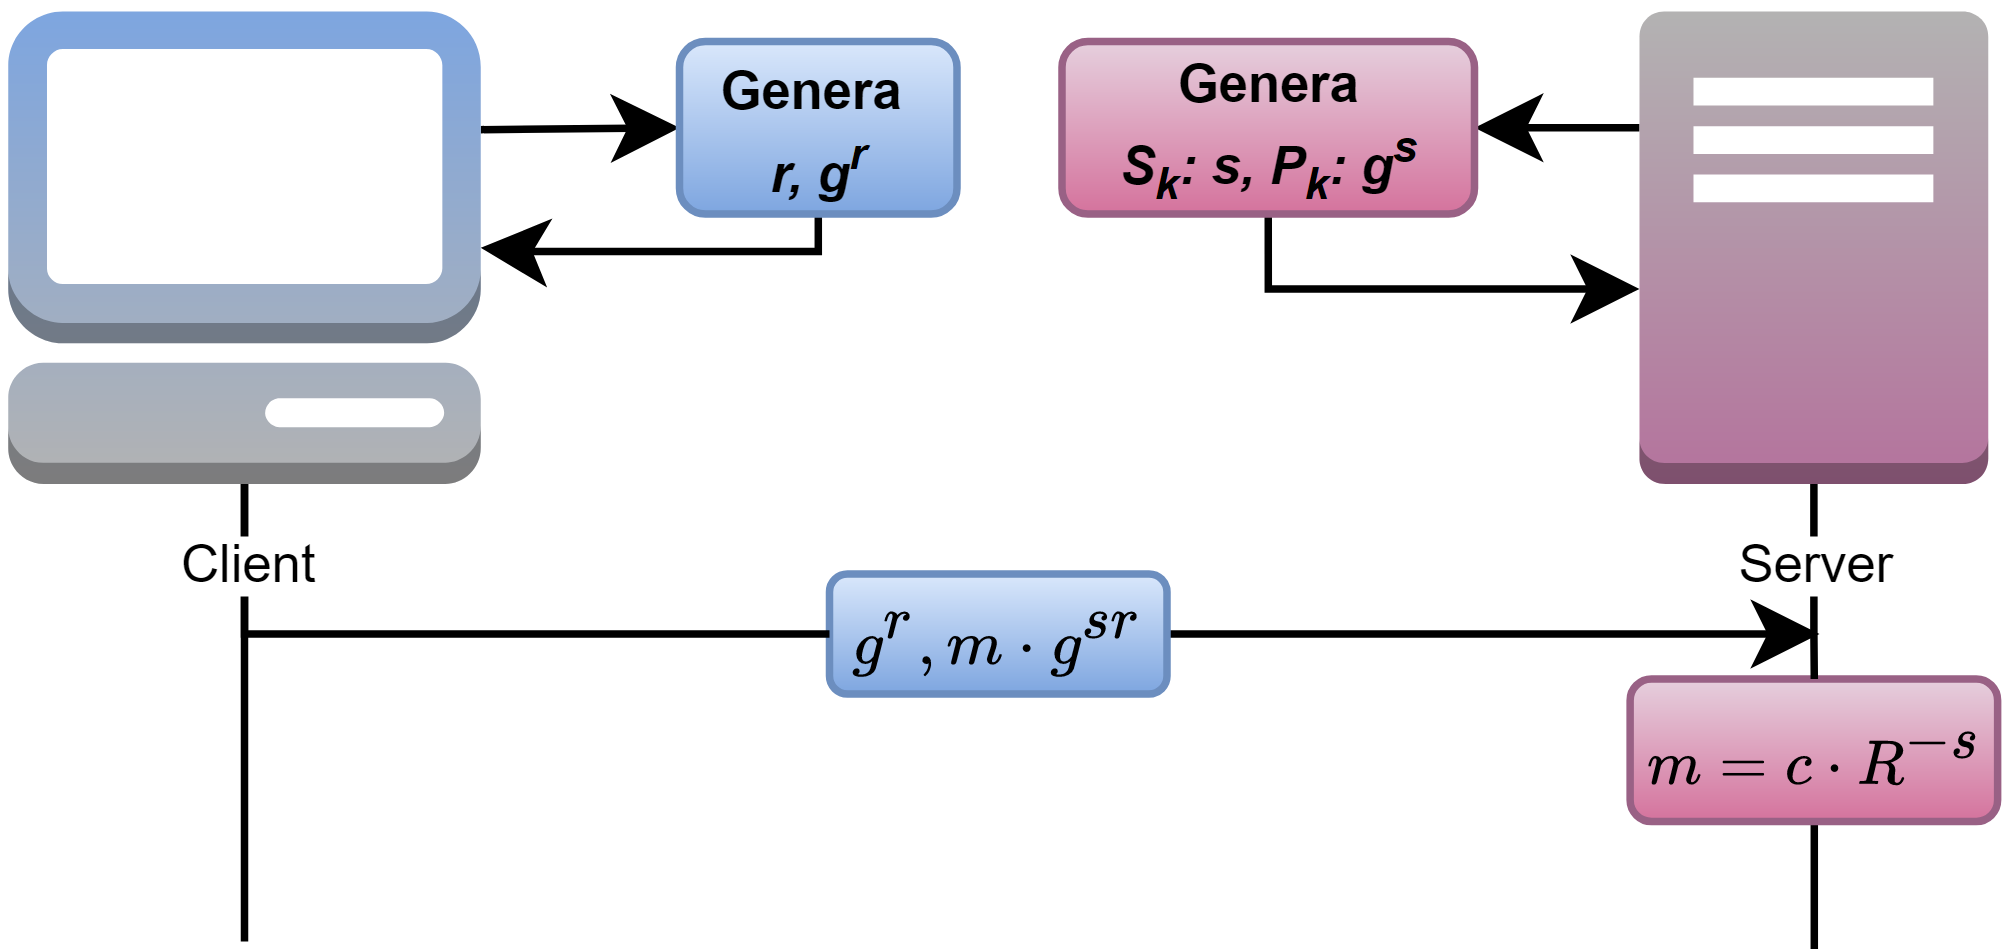
\includegraphics[width=0.7\textwidth]{image/threshold/elgamal.png}
    \caption{ElGamal scheme}
    \label{fig:elgam}
\end{figure}
\begin{note}
Nell'esempio possiamo vedere come lo schema è molto simile a DH, in quanto $g^s,g^r$ sono i coefficienti pubblici (rispettivamente per la chiave privata e per il ciphertext). $s,r$ sono segreti noti esclusivamente al ricevente e al trasmittente rispettivamente, quindi \textbf{non c'è modo} per chiunque di ricostruire $g^{sr}$.\\
Tra l'altro, $r$ è un segreto \textbf{effimero} che viene generato \textit{on-the-fly}.
\end{note}
\section{Asymmetric Ciphers and Hybrid Encryption}
\begin{wrapfigure}{r}{0.4\textwidth}
\centering
    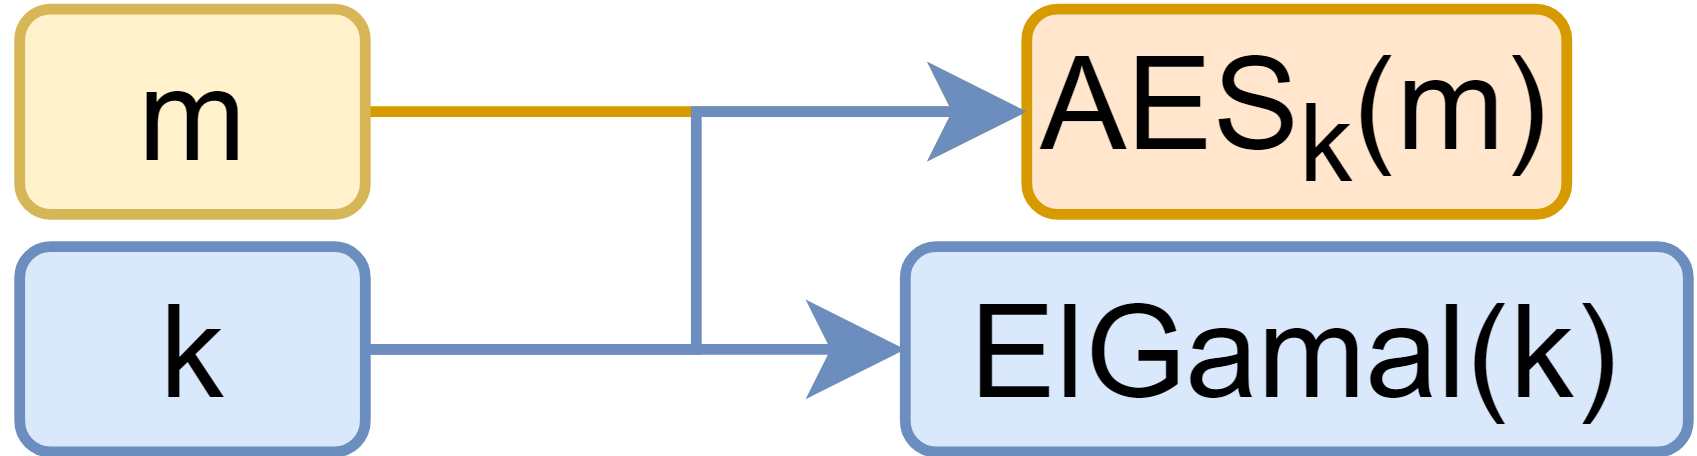
\includegraphics[width=0.38\textwidth]{image/threshold/hybrid.png}
\caption{Hybrid Encryption}
\label{fig:hybrid}
\end{wrapfigure}
I cifratori asimmetrici devono inviare messaggi che siano all'interno del gruppo che viene generato dal numero primo scelto. Ovviamente, i messaggi possono essere molto più grandi della dimensione scelta per il numero primo $p$. Servono quindi schemi che possano lavorare fianco a fianco con quelli classici (es: AES) che si occuperanno di cifrare il messaggio, mentre i primi cifreranno la chiave con cui il messaggio è stato protetto.\\
Questa modalità caratterizza gli schemi \textbf{\textit{ibridi}}, usati ad esempio nei sistemi 5G quando l'utente deve necessariamente comunicare il proprio \textbf{IMSI} (la propria identità digitale). Un modo per creare uno schema ibrido è usare \textbf{ElGamal}.

\begin{example}[ IMSI share in Modern Cell Network]
Consideriamo una SIM all'interno della quale è stata scritta la public-key della Home Network $g^{HN}$ e la chiave privata dell'utente $x$.\\
Facciamo uno scambio di chiavi:
\begin{enumerate}
    \item Viene generata la chiave pubblica $g^x$.
    \item Viene derivata la chiave di cifratura con $K=HKDF(g^{HN\cdot x})$.
    \item L'utente invia in modo cifrato il suo \textbf{SUPI}\footnote{La nuova versione dell'IMSI.} con $AES_K(SUPI)$ insieme ad un HMAC per la verifica e la sua chiave pubblica.
    \item In ricezione la HN prende il pacchetto $(g^x,AES_K(SUPI),HMAC(AES_K(SUPI)))$ e usa $g^x$ per ricostruire la chiave con $K=HKDF(g^{HN\cdot x})$.
    \item Viene usata la chiave ricostruita per decifrare e fare la verifica di integrità.
\end{enumerate}
\end{example}

\subsection{Threshold ElGamal}
ElGamal è uno schema che torna utile anche per quei casi in cui vogliamo rendere la decrittazione di un messaggio possibile \textbf{solo se} un certo numero di persone riceventi coopera. Una prima idea di questo schema potrebbe essere la seguente:
\begin{enumerate}
    \item Utilizzando uno schema di Pedersen (t,n) vengono condivisi share della chiave privata $S$.
    \item Ricostruisco la chiave privata $S$ quando le $t$ parti sono riunite.
\end{enumerate}
Il problema di questo schema è che una volta che la chiave viene ricostruita è disponibile a tutti e qualsiasi cosa potrà essere decifrato da quel momento in poi.
\begin{problem}
\textbf{Possiamo decifrare un messaggio e garantire confidenzialità per qualsiasi altri messaggi?}
\end{problem}
La risposta è ovviamente si e possiamo pensare di usare uno schema ElGamal-like, dove la chiave pubblica è generata on-the-fly per ogni nuovo messaggio e quindi in decryption il denominatore sarà qualcosa del tipo $g^{r_is}$ per il messaggio \textit{i-esimo}. Lo schema corretto è il seguente:
\begin{definition}[threshold ElGamal]\label{def:treshelg}
Consideriamo uno schema (t,n). Sia $p$ strong-prime, con $q$ large prime. Sia $g\in QR_p$ il generatore del sottogruppo. Presa secret-key $s\in\mathbb{Z}_q$ random, la pub-key è $h=g^s\bmod{p}$.\\
\textbf{Come Dealer:}
\begin{enumerate}
    \item Genero polinomio $p(x)\bmod{q}$ di ordine $t-1$ e invio ad ogni parte $(x_i, y_i)$ con $y_i=p(x_i)\bmod{q}$.
    \item Faccio trasmissione del messaggio $m$ tramite ElGamal (\cref{def:elgam}), inviando 
    \[ (R,c)=(g^r,m\cdot h^r)\bmod{p}\]
    con $r\in\mathbb{Z}_q$
\end{enumerate}
\textbf{Come Receiver:}
\begin{enumerate}
    \item Estraggo chiave pubblica $g^r$ dal messaggio ricevuto.
    \item Calcolo il coefficiente di Lagrange:
    \[\Lambda_{x_i}=\prod_{\text{shares} x_k\ne x_i}\frac{-x_k}{x_i-x_k}\bmod{q}\]
    \item Calcolo l'esponenziale dello share per la decrittazione: $w_i=(g^r)^{y_i\Lambda_i}\bmod{p}$
    \item Raccogliendo $t$ shares, possiamo ricostruire la chiave di decrittazione:
    \[\prod_{i=1}^{t}w_i=\prod_{i=1}^{t}(g^r)^{y_i\Lambda_i}=(g^r)^{\sum_{i=1}^{t}{y_i\Lambda_i}}=(g^r)^s=g^{rs}\bmod{p}\]
    \item La decrittazione è possibile: 
    \[m=c\cdot R^{-s}=\frac{c}{(g^r)^s}=\frac{m\cdot h^r}{g^{rs}}=\frac{m\cdot g^{rs}}{g^{rs}}\bmod{p}\]
\end{enumerate}
\begin{remark}
    La secret-key $s$ non viene \textbf{mai rivelata/ricostruita} poiché per ogni messaggio $m$ viene generata una nuova nonce $r$ e quindi la \textbf{chiave di decifratura} $g^{rs}$ sarà \textbf{sempre diversa}.
\end{remark}
\end{definition}
\section{Threshold Signature}
La threshold signature è uno use-case molto più importante rispetto alla threshold encryption perché permette a $t$ membri di un gruppo di $n$ elementi di firmare un messaggio. Questo consente di fare cose come:
\begin{itemize}
    \item Verifica della validità della firma da molteplici fonti.
    \item Un membro del gruppo può essere certificato dagli altri $t$ membri.
    \item Posizionare un segreto in più di una CA.
    \item Impossibilità di creare una firma se meno di $t$ utenti non cooperano.
\end{itemize}
Le uniche accortezze a cui bisogna stare attenti sono le seguenti: 
\begin{itemize}
    \item Riutilizzare sistemi di firma esistenti.
    \item La dimensione della firma non deve scalare con il numero di partecipanti.
\end{itemize}
Uno dei sistemi di firma che possono essere fatti è tramite RSA, vediamone lo schema:
\begin{definition}[RSA Signature]\label{def:rsasign}
\begin{enumerate}
    \item Scegliere numeri primi \textbf{grandi} $p,q$ tale che $N=pq$. Allora $\phi(N)=(p-1)(q-1)$
    \item Scelgo public-key $e$ coprimo con $\phi(N)$ e calcolo la secret-key $d=e^{-1}\bmod\phi(N)$
    \item \textbf{Firmo:} \{$m,H(m)^d$\}
    \item \textbf{Controllo la firma:} \{$H(M)=(H(m)^d)^e$\}
\end{enumerate}
\end{definition}
Per estendere questo schema ad uno a soglia, potremmo procedere con il solito approccio:
\begin{enumerate}
    \item Come dealer, genero un polinomio $f(x)$ tale che $f(0)=d$.
    \item Invio lo share $(x_i,y_i=f(x_i))\bmod\phi(N)$
    \item Invio messaggi firmati $\{m, H(m)\}$
    \item Share della firma: $H(m)^{y_i\Lambda_i}\bmod{N}$
    \item Verifico firma: $\prod H(m)^{y_i\Lambda_i}=H(m)^{\sum y_i\Lambda_i}=H(m)^d$
\end{enumerate}
Se provassimo ad eseguire questo schema, troveremmo che non funziona, perché:
\begin{proof}
La parte i-esima deve calcolare: $H(m)^{y_i\Lambda_i}\bmod{N}$, dove 
\[\Lambda_{x_i}=\prod_{\text{shares} x_k\ne x_i}\frac{-x_k}{x_i-x_k}=\frac{\alpha_{x_i}}{\beta_{x_i}}=\textcolor{red}{\alpha_{x_i}\beta_{x_i}^{-1}}\]
Quindi, la firma sullo share sarebbe:
\[H(m)^{y_i\Lambda_i}\bmod{N}=H(m)^{y_i\alpha_{x_i}\beta_{x_i}^{-1}}\bmod{N}\]
Tuttavia, il funzionamento di RSA è dovuto al fatto che l'esponenziale è calcolato rispetto una potenza \textbf{intera}, quindi non possiamo fare l'esponenziale di una frazione. Tra l'altro, questo significherebbe calcolare $H(m)^\frac{1}{e}$ il che significherebbe \textbf{rompere RSA} perché la sua sicurezza \textbf{risiede} nel fatto che \textbf{non possiamo calcolare} $e^{-1}$ senza conoscere $\phi(n)$ perché equivarrebbe a \textbf{trovare una fattorizzazione}.
\end{proof}
\begin{remark}
Se il termine $\beta$ fosse pari, non potremmo neanche calcolare l'inversa modulare.
\end{remark}
\begin{note}
Uno schema (n,n), non avendo la frazione (no termine di Lagrange), avrebbe funzionato.\pagebreak
\begin{definition}[RSA (n,n) Signature]\label{def:nnrsasign}
\begin{itemize}
    \item \textbf{RSA Setup:} seleziona $p,q$ large primes tale che
    \begin{equation*}
        \begin{aligned}
            &N=p\cdot q\longrightarrow \phi(N)=(p-1)(q-1)\\
            &1<e<\phi(N)\,:\,\gcd(e,\phi)=1\longrightarrow d=e^{-1}\bmod{\phi}
        \end{aligned}
    \end{equation*}
    \item \textbf{Dealer:}
    \begin{itemize}
        \item genera $n$ shares truly random tale che:
        \[y_i=
        \begin{cases}
            r_i\bmod{\phi}&\text{if $i\ne n$}\\
            d-\sum_{i=1}^{n}r_i\bmod{\phi}&\text{if $i=n$}
        \end{cases}    
        \]
        \item invia ad ogni peer il relativo share.
    \end{itemize}
    \item \textbf{Receiver:} Ogni peer esegue
    \begin{itemize}
        \item Dato il messaggio $m$ calcola $H(m)$.
        \item Si crea uno \textbf{share della firma}: $w_i=H(m)^{y_i}\bmod{N}$
        \item Si comunica lo share agli altri peer.
   \end{itemize}
   \item \textbf{Verifica della firma:} ogni peer raccoglie gli share delle altre parti e
   \begin{itemize}
       \item Si ricostruisce la firma condivisa:
       \[
       \prod_{i=1}^{n}w_i=H(m)^{\sum_{i=1}^{n}y_i}=H(m)^{d-\sum_{i=1}^{n}r_i+\sum_{i=1}^{n}r_i}=H(m)^d\bmod{N}
       \]
       \item Si verifica la correttezza della firma calcolando $H(m)$ e verificando che
       \[
       H(m)=(H(m)^d)^e\bmod{N}
       \]
   \end{itemize}
\end{itemize}
\end{definition}
\end{note}
Vediamo una soluzione al problema, proposta da Victor Shoup\footnotetext{\href{https://www.iacr.org/archive/eurocrypt2000/1807/18070209-new.pdf}{Victor Shoup - RSA Threshdol}}:
Consideriamo uno scenario con $L$ player e assumiamo come sempre che lo share sia del tipo $x_i=i$. La base di lagrange che andrà calcolata nel caso di uno schema $(L,L)$ sarà del tipo:
\begin{equation}\label{eq:lbasersa}
\Lambda_{i}=\prod_{\text{shares} k\ne i}\frac{x-k}{i-k}=\frac{\text{something}(x)}{(i-1)(i-2)\dots(i(i-1))(i-(i+1))\dots(i-L)}
\end{equation}
\begin{remark}
Si può vedere che il denominatore di \cref{eq:lbasersa} è \textbf{sicuramente} un \textbf{divisore} di $i!(L-i)!$ in quanto la \textbf{prima metà} è proprio $(i-1)!$ e la \textbf{seconda metà} è $(L-i)!$. Se adesso consideriamo il coefficente binomiale $\binom{L}{i}=\frac{L!}{i!(L-i)!}$ possiamo vedere che $L!\Lambda_i=\overline{\Lambda_i}(x)$ è sicuramente un numero intero porta a 1 il denominatore di $\Lambda_i$.
\end{remark}
Quindi lo schema della soluzione potrebbe essere il seguente:
Come \textbf{Dealer}:
\begin{enumerate}
    \item Scegliere numeri primi \textbf{grandi} $p,q$ tale che $N=pq$. Allora $\phi(N)=(p-1)(q-1)$.
    \item Scelgo public-key $e$ coprimo con $\phi(N)$ e calcolo la secret-key $d=e^{-1}\bmod\phi(N)$.
    \item Genero polinomio $f(x)$ di grado $t-1$ tale che $f(0)=d$.
    \item Invio share i-esimo: $(i,y_i)\bmod\phi(N)$
    \item Firmo lo share\footnotemark come: $H(m)^{y_i\overline{\Lambda}_{x_i}}\bmod N$ dove
    \[\overline{\Lambda}_{x_i}=L!\Lambda_i=L!\prod_{\text{shares} x_k\ne x_i}\frac{-x_k}{x_i-x_k}\]
    \footnotetext{Adesso è possibile poiché esponente intero e non serve più l'inversa.}
\end{enumerate}
Come \textbf{Verifier} per ricostruire la firma faccio:
\[\prod H(m)^{y_i\overline{\Lambda}_{x_i}}=H(m)^{L!\sum y_i\Lambda_{x_i}}=H(m)^{d\cdot L!}\bmod{N}\]
\begin{note}
\textbf{Problema: la firma creata non è la firma}, ma la firma \textbf{elevata} ad una \textbf{costante}, $L!$. \textbf{Potremmo} decidere di dividere per la stessa costante, ma torneremmo al caso precedente, introducendo il calcolo dell'inversa in modulo $\phi(N)$, che \textbf{non possiamo fare}.\end{note}
\subsection{RSA Common Modulus Attack}
La nota scritta prima non è necessariamente vera, poiché l'approccio "alla Shoup" descritto prima non è completo.\\
Introduciamo innanzitutto una vulnerabilità di RSA: 
\begin{proposition}[Modulus Reuse]
In RSA, \textbf{mai riutilizzare} due volte lo stesso modulo $N$ per due chiavi pubbliche differenti.
\end{proposition}
Questo può succedere quando su diversi sistemi di cifratura (ad esempio due siti diversi gestiti dalla stessa entità) utilizziamo lo stesso numero primo $N$ per due chiavi pubbliche differenti. Lo scenario è abbastanza comune, in quanto la parte difficile di RSA è trovare $p,q$ che fattorizzano $N$, mentre la parte facile è derivare quante chiavi pubbliche vogliamo, purché $e_i$ sia coprima con $\phi(N)=(p-1)(q-1)$ e $p-1, q-1$ siano \textbf{strong-primes}.\\
Utilizziamo un esempio per esprimere il concetto del \textbf{Common Modulus Attack}
\begin{theorem}[RSA Common Modulus Attack]\label{thm:rsacomm}
\noindent\begin{itemize}
    \item Supponiamo che Alice cifri un messaggio $m$ con la public-key $e_a$ e che Bob cifri lo \textbf{stesso} messaggio $m$ con una chiave pubblica $e_b$.
    \item Supponiamo anche che il numero $N$ su cui calcoliamo il modulo sia lo stesso.\\
    \begin{remark}
    Questo implica che \textbf{le chiavi pubbliche sono coprime tra loro} in quanto \textbf{devono} essere \textbf{coprime con $\phi(N)$}.  
    \end{remark}
\end{itemize}
Si può dimostrare che tramite \textbf{Ext. Euclidean Algorithm} si può decryptare il messaggio, ovvero: Troviamo $r,s$ \textbf{interi} tale che $e_a\cdot r+e_b\cdot s=1$
\end{theorem}
\begin{proof}
Applichiamo l'Extended-GCD al nostro caso per trovare $r,s$ interi e prendiamo i due ciphertext $c_1=m^{e_a}, c_2=m^{e_b}$.\\
Adesso calcoliamo:
\begin{equation}\label{eq:rsamod}
    c_1^r\cdot c_2^s=(m^{e_a})^r+(m^{e_b})^s=m^{e_a\cdot r+e_b\cdot s}=m
\end{equation}
E abbiamo decryptato il messaggio senza conoscere la chiave di decrittazione/privata.
\end{proof}\pagebreak
\begin{remark}\textbf{RSA Common Modulus Attack} è possibile quando:
\begin{itemize}
    \item due sistemi RSA usano \textbf{lo stesso modulo $N$} per due \textbf{differenti coppie} $(e,d)$ e \textbf{viene cifrato lo stesso messaggio}
\end{itemize}
\end{remark}
Utilizziamo ora l'\cref{eq:rsamod} a nostro vantaggio per eliminare il fattore $L!$ (ovvero il numero massimo di player nello schema).
\begin{note}
    Nella pratica, sarebbe possibile usare anche un altro numero al posto di $L!$, purché il termine usato permetta di ottenere tutti esponenziali interi.
\end{note}
\begin{definition}[Shoup - RSA Threshold]\label{def:shouprsa}
Come \textbf{Dealer}:
\begin{enumerate}
    \item Scegliere numeri primi \textbf{grandi} $p,q$ tale che $N=pq$. Allora $\phi(N)=(p-1)(q-1)$.
    \item Scelgo public-key $e$ coprimo con $\phi(N)$ e calcolo la secret-key $d=e^{-1}\bmod\phi(N)$.
    \item Genero polinomio $f(x)$ di grado $t-1$ tale che $f(0)=d$.
    \item Invio share i-esimo: $(i,y_i)\bmod\phi(N)$
    \item Firmo lo share\footnotemark come: $H(m)^{y_i\overline{\Lambda}_{x_i}}\bmod N$ dove
    \[\overline{\Lambda}_{x_i}=L!\Lambda_i=L!\prod_{\text{shares} x_k\ne x_i}\frac{-x_k}{x_i-x_k}\]
    \item La firma pubblicata è però $H(m)^d$, ottenuta effettuando i passi nell'osservazione successiva.
    \footnotetext{\textsuperscript{\thefootnote}Adesso è possibile poiché esponente intero e non serve più l'inversa.}
\end{enumerate}
Come \textbf{Verifier} per ricostruire la firma faccio:
\[\prod H(m)^{y_i\overline{\Lambda}_{x_i}}=H(m)^{L!\sum y_i\Lambda_{x_i}}=H(m)^{d\cdot L!}\bmod{N}\]
Adesso per ottenere la firma esatta ed effettuare la verifica, applico i seguenti passi:\\
\begin{remark}
Sia ora $L!=\Delta$. Allora:
\[H(m)^{d\cdot L!}=H(m)^{d\Delta}=v^{\Delta}\]
Osserviamo che la quantità $H(m)=[H(m)^{d}]^e=v^e$ è nota\footnotemark.
\footnotetext{\textsuperscript{\thefootnote}La chiave di cifratura $e$ è pubblica e può essere usata.}
Poiché vogliamo $H(m)^d=v$ per controllare la firma, usando l'RSA Common Modulus Attack (\cref{thm:rsacomm}) troviamo $v$, \textbf{se $\Delta$ ed $e$ sono coprimi\footnotemark}:
\begin{itemize}
    \item tramite $ExtGCD(e,\Delta)$ troviamo $(r,s)$.
    \item Calcoliamo: $(v^{e})^r\cdot (v^{\Delta})^s=v^{e\cdot r+\Delta\cdot s}=v$
\end{itemize}
\end{remark}
\footnotetext{\textsuperscript{\thefootnote}Questo succede praticamente sempre se $e$ è un numero pimo più grande di $L$. Altrimenti la firma con RSA resta uguale.}
\end{definition}
\begin{remark}Se svolgiamo i calcoli sul sottogruppo dei \textbf{Residui Quadratici} (\cref{def:quadres}) e usiamo primi forti (\cref{eq:strongp}) $p=2p'+1,q=2q'+1$ allora il periodo di $N=pq$ sarà $\phi(N)=(p-1)(q-1)=2p'\cdot2q'=4p'q'$. Il periodo spannato da questo numero è \textbf{molto grande}, anche se non è primo. Quindi non c'è il problema di invertire il modulo a meno di voler invertire un numero del tipo $1/p'$ ma non succede praticamente mai.
\end{remark}
\begin{note}
Schoup dimostrò anche la verificabilità del secret sharing fatto con questa tecnica.
\end{note}
\begin{note}
Il problema che questo schema ha è che \textbf{almeno una} persona nel mondo conosce $\phi(N)$, il Dealer. Questo problema è stato risolto da Foque e Stern, nel 2001. Non lo vediamo, anche perché RSA al giorno d'oggi è obsoleto rispetto ad altri sistemi di sicurezza.
\end{note}
